\chapter{Dizer as horas demanda trabalho}
\label{les:17}

\begin{chapquote}{Lewis Carroll, \textit{Alice no País das Maravilhas}}
\enquote{Oh puxa! Oh puxa! Eu devo estar muito atrasada!}
\end{chapquote}

Costuma-se dizer que os bitcoins são minerados porque milhares de computadores trabalham na solução de problemas matemáticos \textit{muito complexos}. Certos problemas precisam ser resolvidos, e se você calcular a resposta certa, você \enquote{produz} um bitcoin. Embora essa visão simplificada da mineração de bitcoin possa ser fácil de ser transmitida e entendida, ela deixa a desejar em alguns aspectos. Os bitcoins não são produzidos ou criados, e toda esssa experiência não é realmente sobre a solução de problemas matemáticos específicos. Além disso, a matemática não é particularmente complexa. O que é complexo é \textit{dizer as horas} em um sistema descentralizado.

Conforme descrito no whitepaper, o sistema de prova de trabalho (também conhecido como mineração) é uma maneira de implementar um servidor de data/hora distribuído.

\begin{figure}
  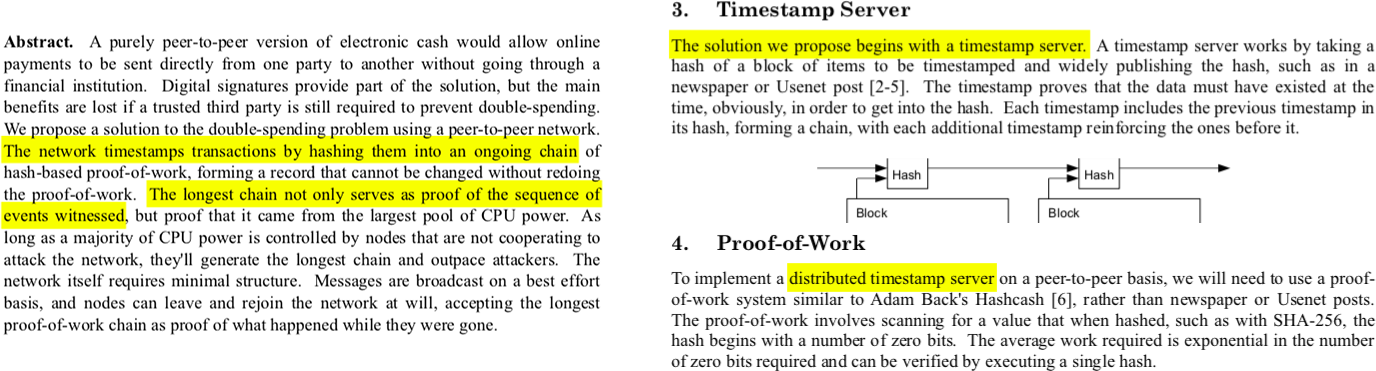
\includegraphics{assets/images/bitcoin-whitepaper-timestamp-wide.png}
  \caption{Trechos do whitepaper. Alguém disse timechain?}
  \label{fig:bitcoin-whitepaper-timestamp-wide}
\end{figure}

Quando aprendi como o Bitcoin funciona, também pensei que a prova de trabalho era ineficiente e um desperdício. Depois de um tempo, comecei a mudar minha perspectiva sobre o consumo de energia do Bitcoin~\cite{gigi:energy}. Parece que a prova de trabalho ainda é muito mal compreendida, mesmo no ano 10 DB (depois do Bitcoin).

Uma vez que os problemas a serem resolvidos na prova de trabalho são criados, muitas pessoas parecem acreditar que este é um trabalho \textit{inútil}. Se o foco for puramente o cálculo, essa é uma conclusão razoável. Mas o Bitcoin não é sobre computação. É sobre \textit{concordar independentemente sobre ordem das coisas}.

A Prova de trabalho é um sistema no qual todos podem validar o que aconteceu e em que ordem aconteceu. Essa validação independente é o que leva ao consenso, um acordo individual entre várias partes sobre quem possui o quê.

Em um ambiente radicalmente descentralizado, não podemos nos dar ao luxo de ter um tempo absoluto. Qualquer relógio introduziria uma terceira parte confiável, um ponto central no sistema que deveria ser confiada e poderia ser atacado. \enquote{O tempo é a raiz do problema}, como Grisha Trubetskoy aponta~\cite{pow-clock}. E Satoshi resolveu esse problema de forma brilhante implementando um relógio descentralizado por meio de uma blockchain de prova de trabalho. Todos concordam de antemão que a cadeia com a maior quantidade de trabalho é a fonte da verdade. É por definição o que realmente aconteceu. Este acordo é o que agora é conhecido como consenso de Nakamoto.

\begin{quotation}\begin{samepage}
\enquote{As transações de registro de data e hora da rede, colocando-as em uma cadeia contínua que serve como prova da sequência dos eventos testemunhados.}
\begin{flushright} -- Satoshi Nakamoto\footnote{Satoshi Nakamoto, Whitepaper do Bitcoin~\cite{whitepaper}}
\end{flushright}\end{samepage}\end{quotation}

Sem uma maneira consistente de saber as horas, não há uma maneira consistente de saber o antes e o depois. Uma ordenação confiável é impossível. Como mencionado acima, o consenso de Nakamoto é o jeito do Bitcoin dizer a hora de maneira consistente. A estrutura de incentivos do sistema produz um relógio probabilístico e descentralizado, utilizando tanto a ganância quanto o interesse próprio dos participantes concorrentes. O fato desse relógio ser impreciso é irrelevante porque a ordem dos eventos acaba sendo inequívoca e pode ser verificada por qualquer pessoa.

Graças à prova de trabalho, o trabalho \textit{e} a validação do trabalho são radicalmente descentralizados. Todos podem entrar e sair à vontade e todos podem validar tudo a qualquer momento. Além disso, todos podem validar o estado do sistema \textit{individualmente}, sem ter que depender de ninguém para isso.

Compreender a prova de trabalho leva tempo. Frequentemente, é contra-intuitivo e, embora as regras sejam simples, elas levam a fenômenos bastante complexos. Para mim, mudar minha perspectiva sobre a mineração ajudou. Útil, não inútil. Validação, não computação. Tempo, não blocos.

\paragraph{O Bitcoin me ensinou que dizer as horas é complicado, especialmente se você estiver em um ambiente descentralizado.}

% ---
%
% #### Through the Looking-Glass
%
% - [Bitcoin's Energy Consumption: A shift in perspective][energy]
%
% #### Down the Rabbit Hole
%
% - [Blockchain Proof-of-Work Is a Decentralized Clock][points out] by Gregory Trubetskoy
% - [The Anatomy of Proof-of-Work][pow-anatomy] by Hugo Nguyen
% - [PoW is efficient][pow-efficient] by Dan Held
% - [Mining][bw-mining], [Controlled supply][bw-supply] on the Bitcoin Wiki
%
% [points out]: https://grisha.org/blog/2018/01/23/explaining-proof-of-work/
% [energy]: 
% [whitepaper]: https://bitcoin.org/bitcoin.pdf
%
% [pow-efficient]: https://blog.picks.co/pow-is-efficient-aa3d442754d3
% [pow-anatomy]: https://bitcointechtalk.com/the-anatomy-of-proof-of-work-98c85b6f6667
% [bw-mining]: https://en.bitcoin.it/wiki/Mining
% [bw-supply]: https://en.bitcoin.it/wiki/Controlled_supply
%
% <!-- Wikipedia -->
% [alice]: https://en.wikipedia.org/wiki/Alice%27s_Adventures_in_Wonderland
% [carroll]: https://en.wikipedia.org/wiki/Lewis_Carroll
